\chapter{FEA data management}
\label{chapter:data-management}

Together with growing complexity of finite element calculations, the importance of management of data produced by the calculations is increasingly emphasized in both industrial and research communities. As information is shared between multiple users, moved from one computer to another, and further transformed to enable different views over the data to enable inpterpretation of the information. Definition of persistent and standard representation of the data is therefore required as well as the corresponding data access system architecture that allows to query the data.

\section{System architecture}
\label{sec:system-architecture}

The prototype implementation of the FEA data management system is designed as a collaborative framework that can be accessed by users from different client devices. Figure \ref{fig:FEA-architecture} depicts the schema of the system architecture. System consists of several independent modules. The FEM calculation itself runs on a remote server as one of micro-services\footnote{TODO: micro-services} along with mesh generation service, results processing service, etc. These services are controlled by the application service that provides interface to the client applications in form of REST-ful web API\footnote{TODO: REST; REST-ful service; REST web API.}.

\begin{figure}[H]
    \centering
    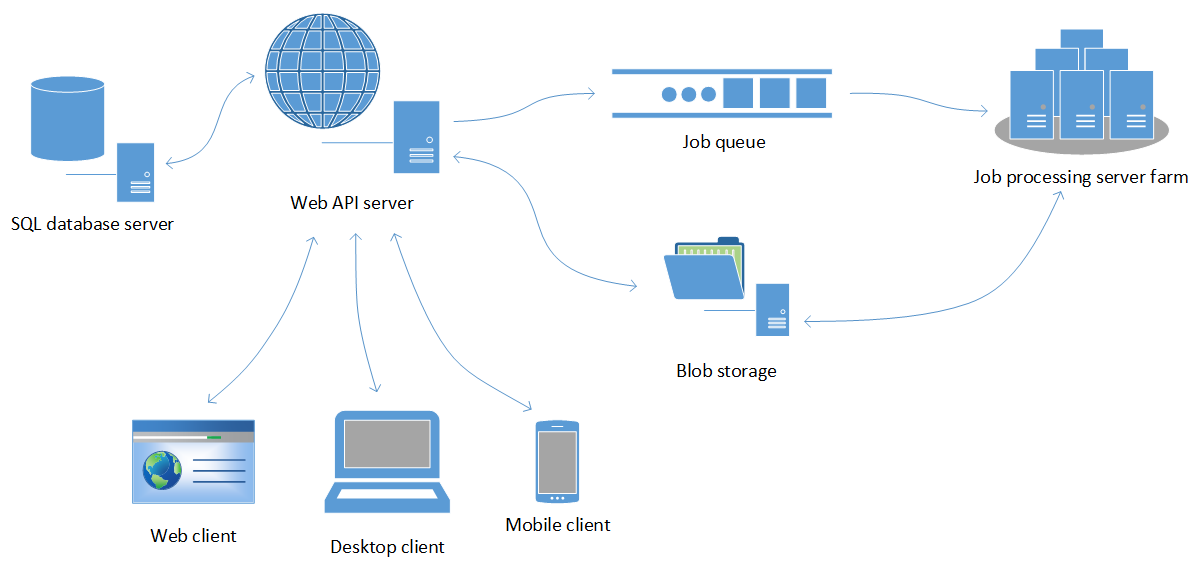
\includegraphics[width=\textwidth]{figures/FEA-architecture}
    \decoRule
    \caption{FEA system architecture.}
    \label{fig:FEA-architecture}
\end{figure}

The architecture relies on an abstraction provided by Platform-as-a-Service\footnote{PaaS. TODO: These services can be carried in a public cloud or on-premises. ...} computing model. No service component is tied directly to a specific machine. Hardware resources are allocated when they are needed by a service infrastructure controller. This makes the scaling and deployment of components easier and allows to focus on the problem domain instead of solving server configuration and networking issues.

The system contains two types of data storage. The relational-database type of storage is intended to store basic project-related data such as description of simulations, links to the simulation resources, information about the owner and other colaborating users, etc. The input to the FEA -- geometrical model, attribute assignments, and analysis parameters -- can also be stored in a relational database. Nevertheless, storing this complex type of information in the SQL database is questionable and has its drawbacks\footnote{TODO: Zminit vyhody i nevyhody. Jake jsou alternativy? No-SQL databaze?}.

The second type of storage is a blob storage used to hold temporary files serving as the input or the output to particular components, especially the mesh generator and the FEM solver. The system is designed to be independent of the solver and mesh generator components, therefore this intermediate step of converting the input to proprietary file format that the components understand is necessary. In the future, it is possible to expect a gradual transition from the file-based approach to the direct connection to the database and query the input model directly. Also, the output of the calculation could be saved directly in the proposed format to represent the results in post-process-ready form.

Workflow diagram in Figure \ref{fig:FEA-workflow} helps to visualize the sequence of FEA steps and the transfer of data between the service components. It also reveals the basic design principle behind the microservice architecture -- Separation of concerns\footnote{Separation of concerns -- design principle for separating system into distinct sections, such that each section addresses a separate concern.}. The vertical bars denote computational intensive tasks performed by the service components. The client side in the diagram represents the presentation layer of the FEA system that the user directly interacts with. In the presentation layer, also called \textit{frontend}, there is spent the vast majority of time by users doing pre- and post-processing of data (which is not depicted in the diagram). The Web API service, also called as \textit{backend}, is the key component that assigns work to other components, serves as an controller for a running analysis and mainly as an interface between the data stored in databases and the client applications.

\begin{figure}[H]
    \centering
    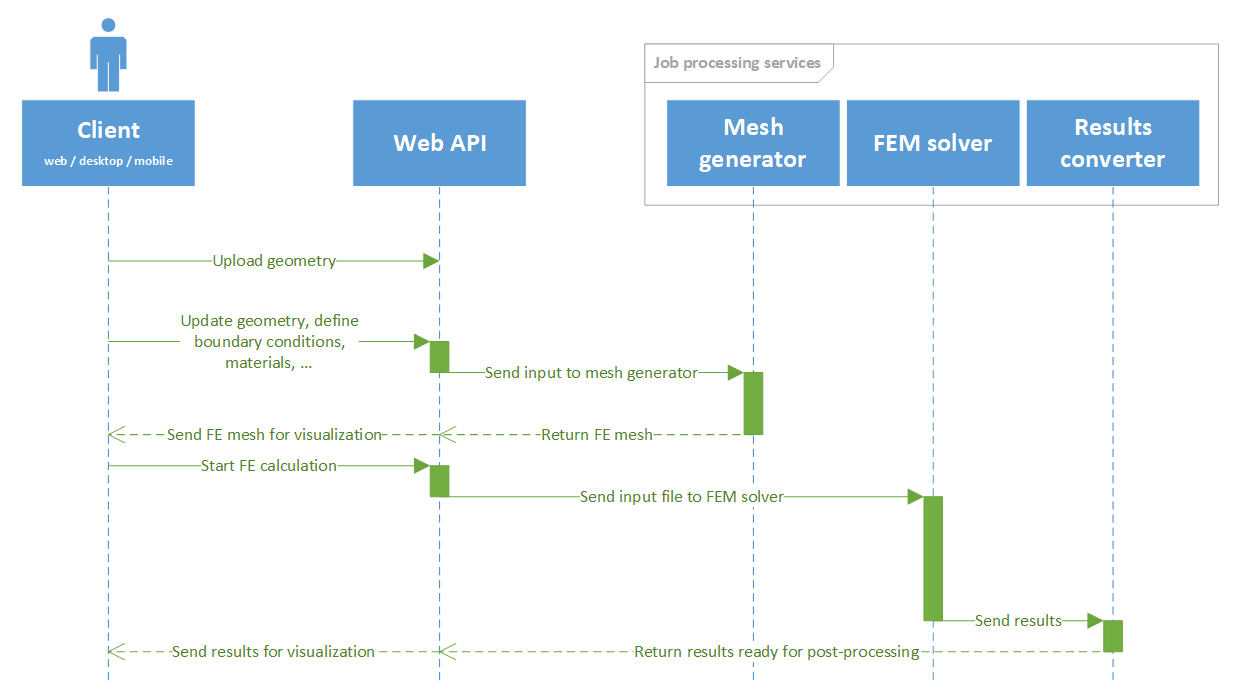
\includegraphics[width=\textwidth]{figures/FEA-workflow}
    \decoRule
    \caption{FEA system workflow.}
    \label{fig:FEA-workflow}
\end{figure}

The prototype implementation of the data management system follows the schema and the workflow depicted in Figures \ref{fig:FEA-architecture} and \ref{fig:FEA-workflow}. The difference is that the pre-processing phase is currently excluded. The focus of the work presented in this thesis is primarily on the post-processing features and the representation of results. Therefore, the results from the existing FEM solver are uploaded into the system and the system converts them to the internal representation suitable for post-processing. To test the prototype implementation of the data management system, two client applications are created. The first is the feature-rich desktop post-processor with the support for Microsoft Windows and Linux operating systems. The second is the simple web application that provides basic control over an analysis and basic post-processing capabilities. Its purpose is mainly to demonstrate the benefits of proposed format for storage of results when post-processing complex FEA. Its web-based implementation allows for truly cross-platform experience without the need for installation and it allows to access the analysis data even from low-end mobile devices.

\section{Project-based data representation} % TODO: prejmenovat tuto kapitolu? Project database schema? Neni to jen o Project-based datech. Mluvi se zde i o vstupnim modelu a o reprezentaci vysledku - vrstvy
\label{sec:project-db-schema}

% Since potentially many users can access the core server to perform structural analysis and to query the analysis results, a project management scheme is needed. The basic premise is that most researchers and engineers typically work independently, while sharing information necessary for collaboration. More importantly, they wish to retain control over the information they make accessible to other members [34]. In the prototype online data access system, a mechanism to perform version control and access control in order to cope with project evolution is implemented. The overall database schema is depicted in Fig. 6. The schema includes a user table and a project table.

Most researchers and engineers typically work independently using their own workstations, while sharing the hardware infrastructure for intensive FEM calculations. The output from the complex analyses are also shared as it would be costly and ineffective if each collaborator had performed her/his own calculations. Since potentially many users can access the server to oversee the analysis and to query the analysis results, a project management scheme is needed. The overall database schema is depicted in Figure \ref{fig:FEA-db-schema}. It is an entity-relationship diagram representing conceptual model that can be mapped on the SQL database model.

\begin{figure}[H]
    \centering
    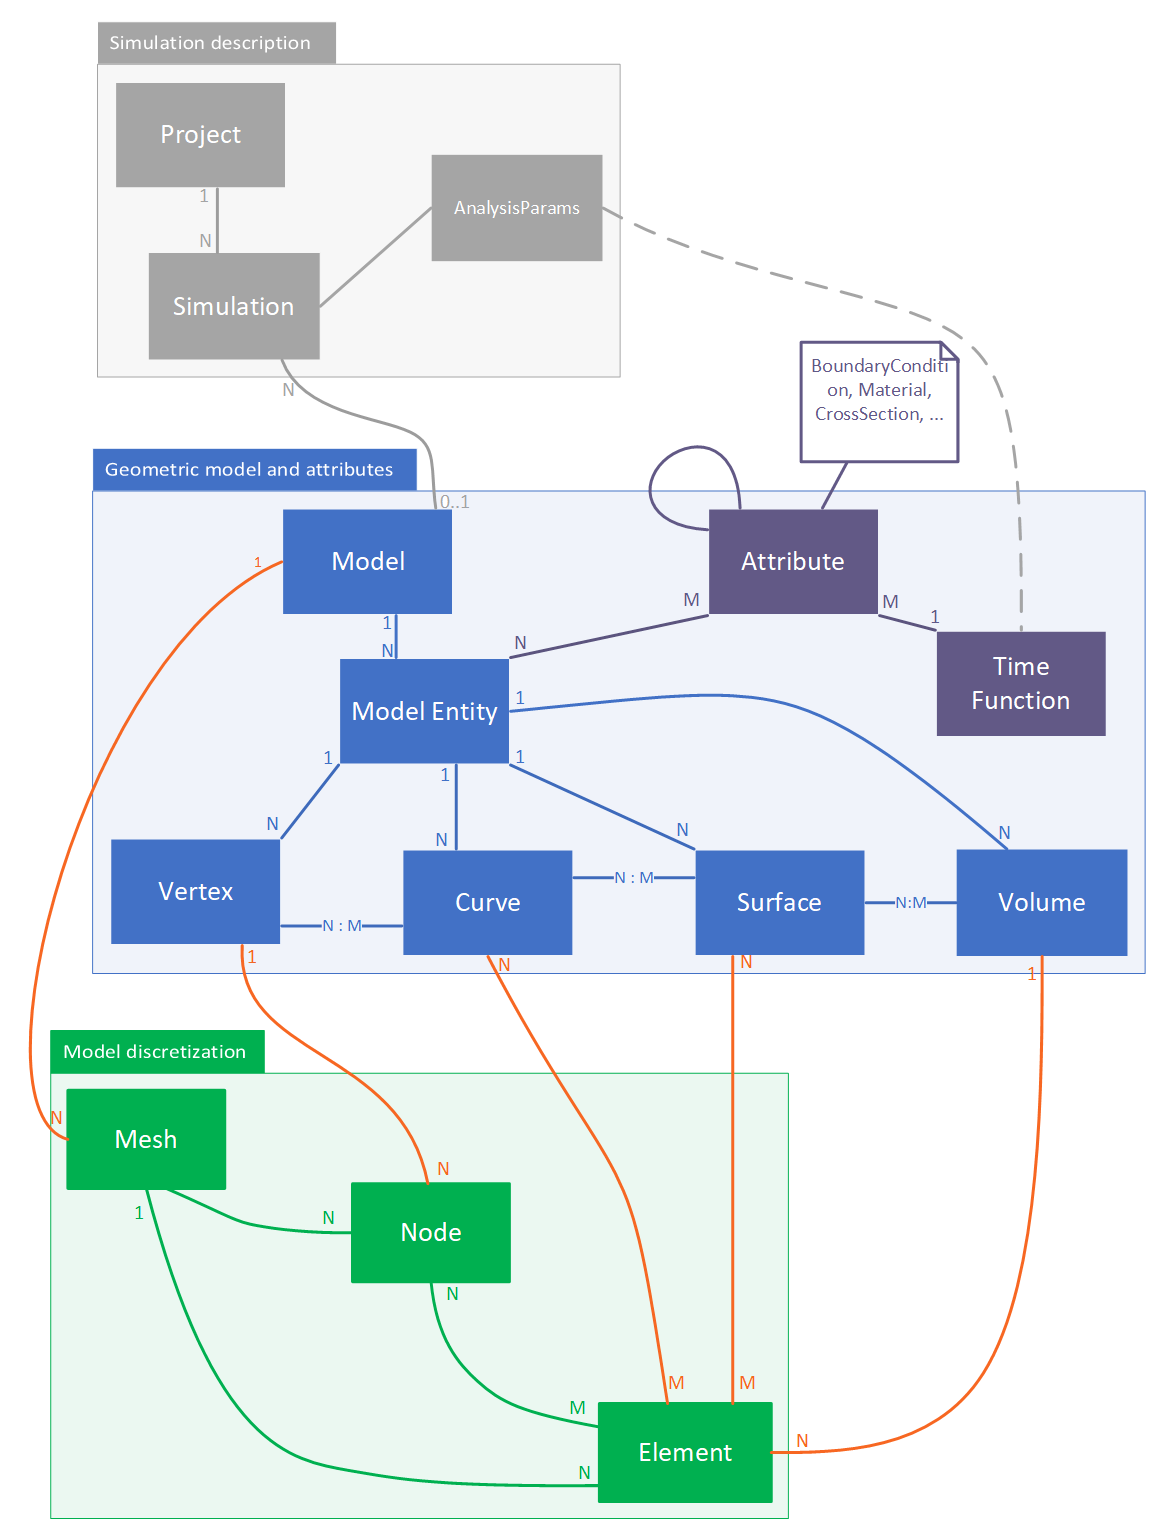
\includegraphics[width=0.8\textwidth]{figures/FEA-database-schema}
    \decoRule
    \caption{Database schema for FEA.}
    \label{fig:FEA-db-schema}
\end{figure}

The Project entity holds the basic information about a set of related analyses. It has name, the owner, and the list of other users that have access permissions. The Project has also relations to the list of simulations. The Simulation entity encapsulates the information about a single finite element analysis. Each simulation can have different input -- geometrical model, attributes, and/or parameters of analysis (e.g. number of time steps). Geometrical model and its discretizations (finite element meshes) can either be stored directly in a relational database or as a custom file in a blob storage.

% Tento model se da prirozene rozsirit o dalsi entity reprezentujici vysledky simulace, viz Figure \ref{fig:FEA-db-schema-results}. Vysledek simulace reprezentuje entita Solution, ktera obsahuje odkaz na vystupni soubory z FEM solveru. Dale je zde entita Layer reprezentujici transformovane vysledky ze solveru do podoby vhodne pro postprocessing. (Vice v nasledujici kapitole.)
% Vstup do FEMu (geometricky model v teto architekture muze byt reprezentovan bud vstupnim souborem vygenerovanym v CADu nebo muze byt ulozen v db)
% In addition to that the desktop postprocessor ma moznost ukladat si data lokalne

% zminit modeller a OOFEM-link, ukazka db modelu
% solution.json
% model attributes: viz clanek FEA with Relational DB, section FEA Data and Dataflow

Figure \ref{fig:FEA-db-schema-results}

% TODO: add User entity to schema?

\begin{figure}[H]
    \centering
    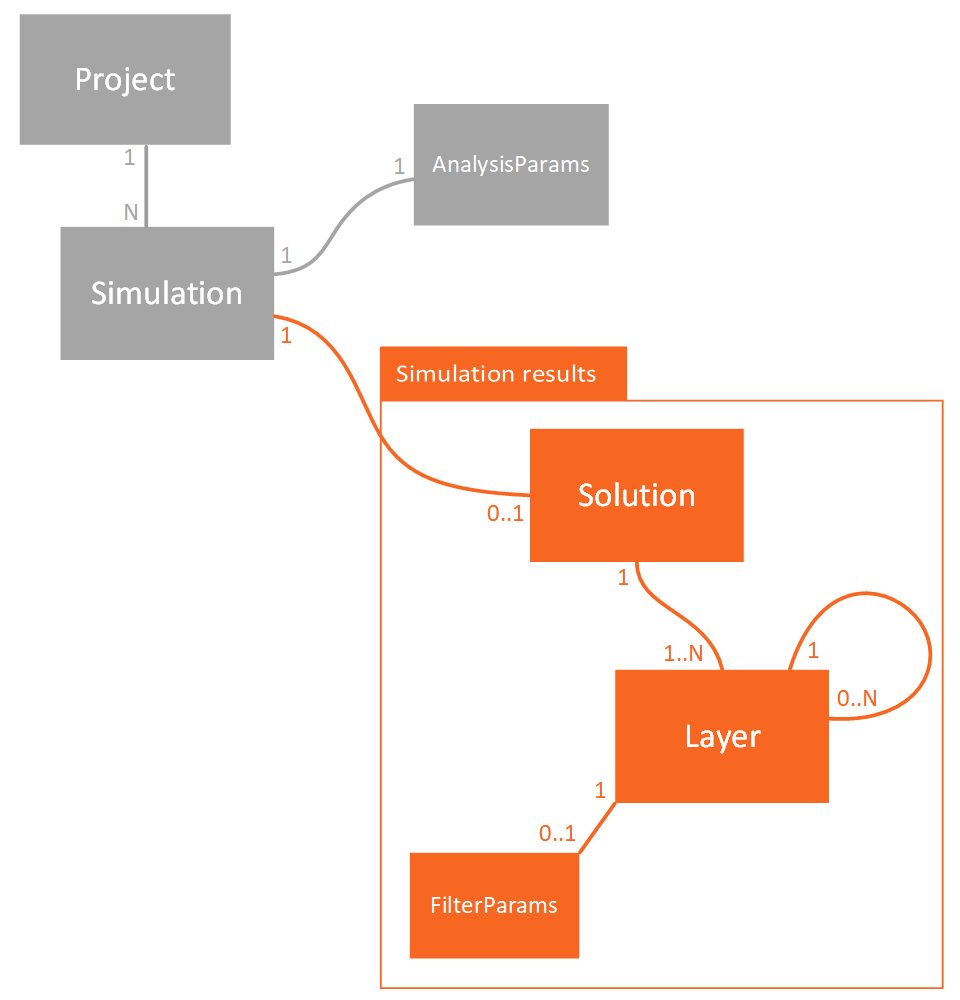
\includegraphics[width=0.6\textwidth]{figures/FEA-database-schema-only-results}
    \decoRule
    \caption{Database schema for FEA with results representation only (without input model).}
    \label{fig:FEA-db-schema-results}
\end{figure}

% model and mesh in persistent storage


\section{Storage format for results}
\label{sec:storage-format}

% Result converter component ma za ukol transformovat vysledky z FEM solveru do mojeho formatu (predpokladam pouziti solver komponenty, ktera ma vlastni proprietarni format, protoze se snazim navrhnout system nezavisly na jednotlivych komponentach)

% Centrem vseho je solution. To muze byt reprezentovano entitou v DB. Pripadne solution.json souborem v pripadne vysledku ulozenych a postprocessovanych lokalne. Hlavni koncept pri postprocessingu ke vrstva - layer - reprezentuje sit konecnych prvku a korespondujici vysledky at uz v uzlech ci v prvcich. Tyto data mohou byt zkompresovana. Vysvetlit, proc mam vic vrstev. Proc nestaci jedna.
% TODO: pridat obrazek stromu vrstev.

Figure \ref{fig:layers-tree}

\begin{figure}[H]
    \centering
    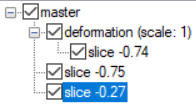
\includegraphics[width=0.5\textwidth]{figures/layers-tree-diagram}
    \decoRule
    \caption{Diagram of layers tree.}
    \label{fig:layers-tree}
\end{figure}

% hodne se inspirovat oznacenymi vetami v clanku FEA-with-relational-DB


% samotny seznam souboru, ktere pouzivam. Nerikat tomu soubory, ale dokumenty? objekty?
% summary.json, mesh.json, attribute.json, and result.json - odkaz do Appendixu na example
% NoSQL DB
% U kazdeho souboru

% konverze z tradicnich souboru do noveho formatu (do budoucna integrovat do solveru); data location Points/Cells/CellPoints, GP extrapolation

% sit je krome vstupu dulezita i u vystupu. je nutne zachovat 1:1 mapovani vysledku na sit

\subsection {Encoding}
% base64, JSON, XML, ...

\subsection {Compression}
% Compression methods: SVD, Wavelet, polynomial functions, ... Kazdou rozepsat, u Wavelet zminit Hilbert curve?
% main features for optimization: key time steps (time step span compression), Randomized SVD, Parallelization, Sparse matrix of details, prenasobeni U matice singularnimi cisly, trochu usetrim pamet, mohu pouzit vzorkovani...

\section{Post-processing}
\label{sec:postprocessing}

% layers, filters, vytvoreni Surface vrstvy pro webovy postprocessor, barevna skala, Remote/Local solutions - neni rozdil, postprocessor je tenky klient, prepinani skalarnich velicin, vektorove veliciny - je treba nacist vice komponent najednou. Dekomprese: prenasobeni matic - staci jeden radek. ...

\section{Implementation details}
\label{sec:implementation-details}
% implementation details; cloud-infrastructure, Azure functions, web frontend, backend providing project info, blob-storage with layer format; command-based console management - popsat prikazy; reference to appendix with storage format examples
% SVD compression using redsvd; How is realized postprocessing of compressed data
% Encoding: converting to text representation, base64, NaN values, ... UTF8

% Webový browser, WebGL, textové pole se zadáváním příkazů, veškeré zpracování příkazů na serveru, na klient se budou posílat jen grafické buffery

% Přidat podkapitolku o implementaci barevné škály (diskrétní, spojitá, isoareas shader)

Figure \ref{fig:results-class-diagram}.

\begin{figure}[H]
    \centering
    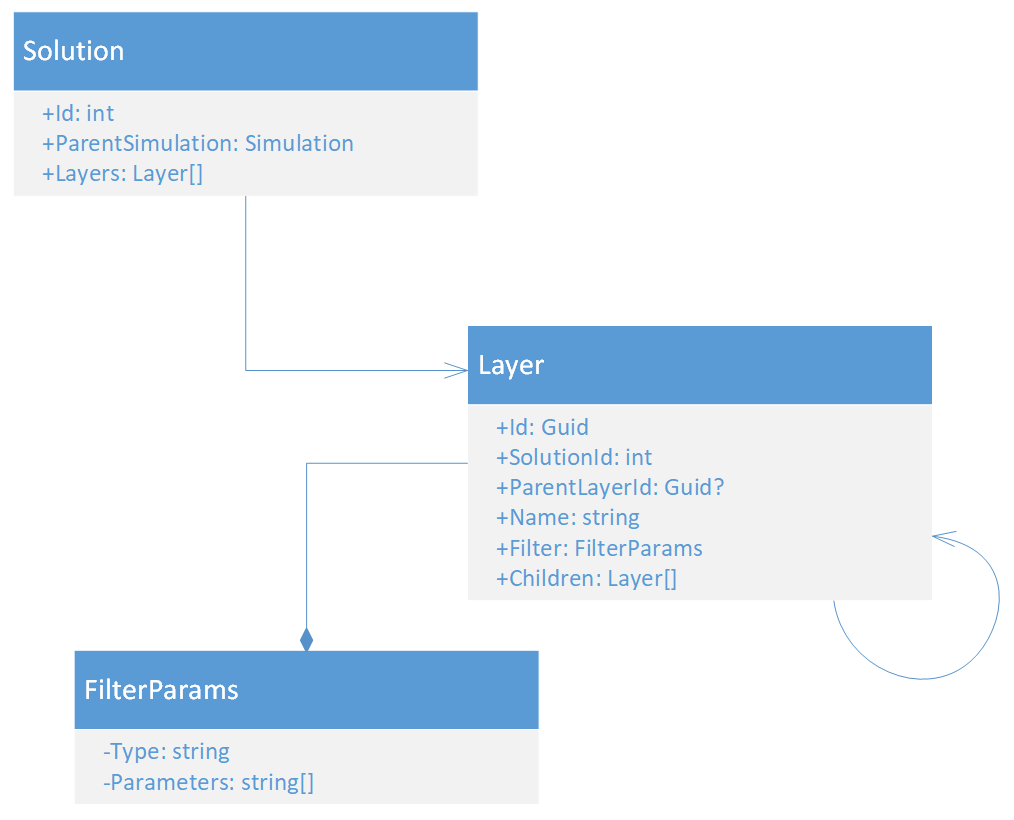
\includegraphics[width=0.7\textwidth]{figures/results-class-diagram}
    \decoRule
    \caption{Class diagram of results representation}
    \label{fig:results-class-diagram}
\end{figure}